\chapter{Experiments and results}

\label{ch:Experiments and results}

\setlength{\parindent}{4em}
\setlength{\parskip}{1em}
\renewcommand{\baselinestretch}{1.5}

\section{Hardware for the experiment}

\hspace{1.5cm} In our project, first we plan how to investigate the EEG data from the subject. There are 2 categories to investigate the data those are software and hardware. When we know like that we go to study how is it different between software and hardware that use in this project and when we already study in it we know that hardware is better than software and we choose it and We plan to design the hardware to use it in experiment.This is materials that we use in our project.

\subsection{EPOC headset by Emotiv\texttrademark}
\hspace{1.5cm} The wireless headset Emotiv EPOC research edition, it records EEG data in 14 channel of International 10-20 Locations system with Sequential sampling rate at 128 per second (2048 Hz internal) with resolution 14 bit (16 bit Analog to digital converter, 2-bit instrumental noise floor discarded), the bandwidth is in range 0.2 to 45 Hz with digital notch filters at 50Hz and 60 Hz

We use this equipment in our experiment to obtain the EEG from the subjects and we use EEG that we can obtain from the user to apply in our project.
\begin{figure}[ht]
	\centering
	\includegraphics[scale = 0.09]{chapter3/36.pdf}
	\caption{EPOC headset by Emotiv\texttrademark}
\end{figure}

\subsection{Arduino Uno}
\hspace{1.5cm} The Arduino Uno is a microcontroller board based on the ATmega328 that is an open source platform. It has 14 input/output pins6 analog inputs, a 16 MHz quartz crystal, a USB connection, a power jack, an ICSP header and a reset button, The USB connection for upload the software into the Arduino and VCC or supply for connecting the peripheral circuit.

In our experiment, we use the arduino uno board to control the hardware which we use to stimuli subjects to get the EEG from subjects to apply it in our project.
\begin{figure}[ht]
	\centering
	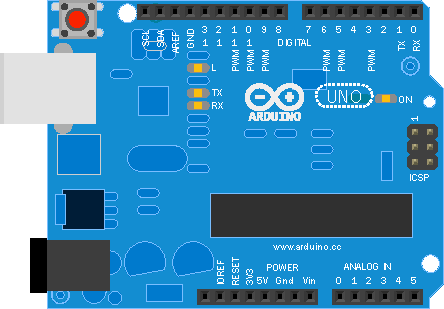
\includegraphics[scale = 0.8]{chapter3/38.pdf}
	\caption{Illustrate of Arduino UNO board}
\end{figure}

\subsection{Gravitech Gerora WS2812S LED}
\hspace{1.5cm} The full-color Light-emitting diode (LED) driver which is use for stimulating the subject has an LED light WS2812 model mounted on. It can chain connected with the same model. It can be controlled by a programmed Arduino. The luminous intensity is 550 to 700 mega candela for red, 1100-1400 mcd for green, and 200-400 mcd for blue.

For this hardware, we use it be flickers to blink the LED that in this board. We can control the frequency, intensity and color of LED. This hardware is controlled by the arduino uno board to stimuli subjects to get the EEG to apply in our project.
\begin{figure}[ht]
	\centering
	\includegraphics[scale = 0.4]{chapter3/37.pdf}
	\caption{Gravitech Gerora LED base on WS2812}
\end{figure}

\subsection{Visual stimulus (ERP)}
\hspace{1.5cm} As the Figure 7.4 show our prototype visual stimulator. It consist of the arduino board and gravitech gerora WS2812 LED board. This stimulator use to stimuli subjects to get EEG. This stimulator blink the light from LED 1 to LED 4 respectively. This stimulator was used in Experiment I.

\begin{figure}[ht]
	\centering
	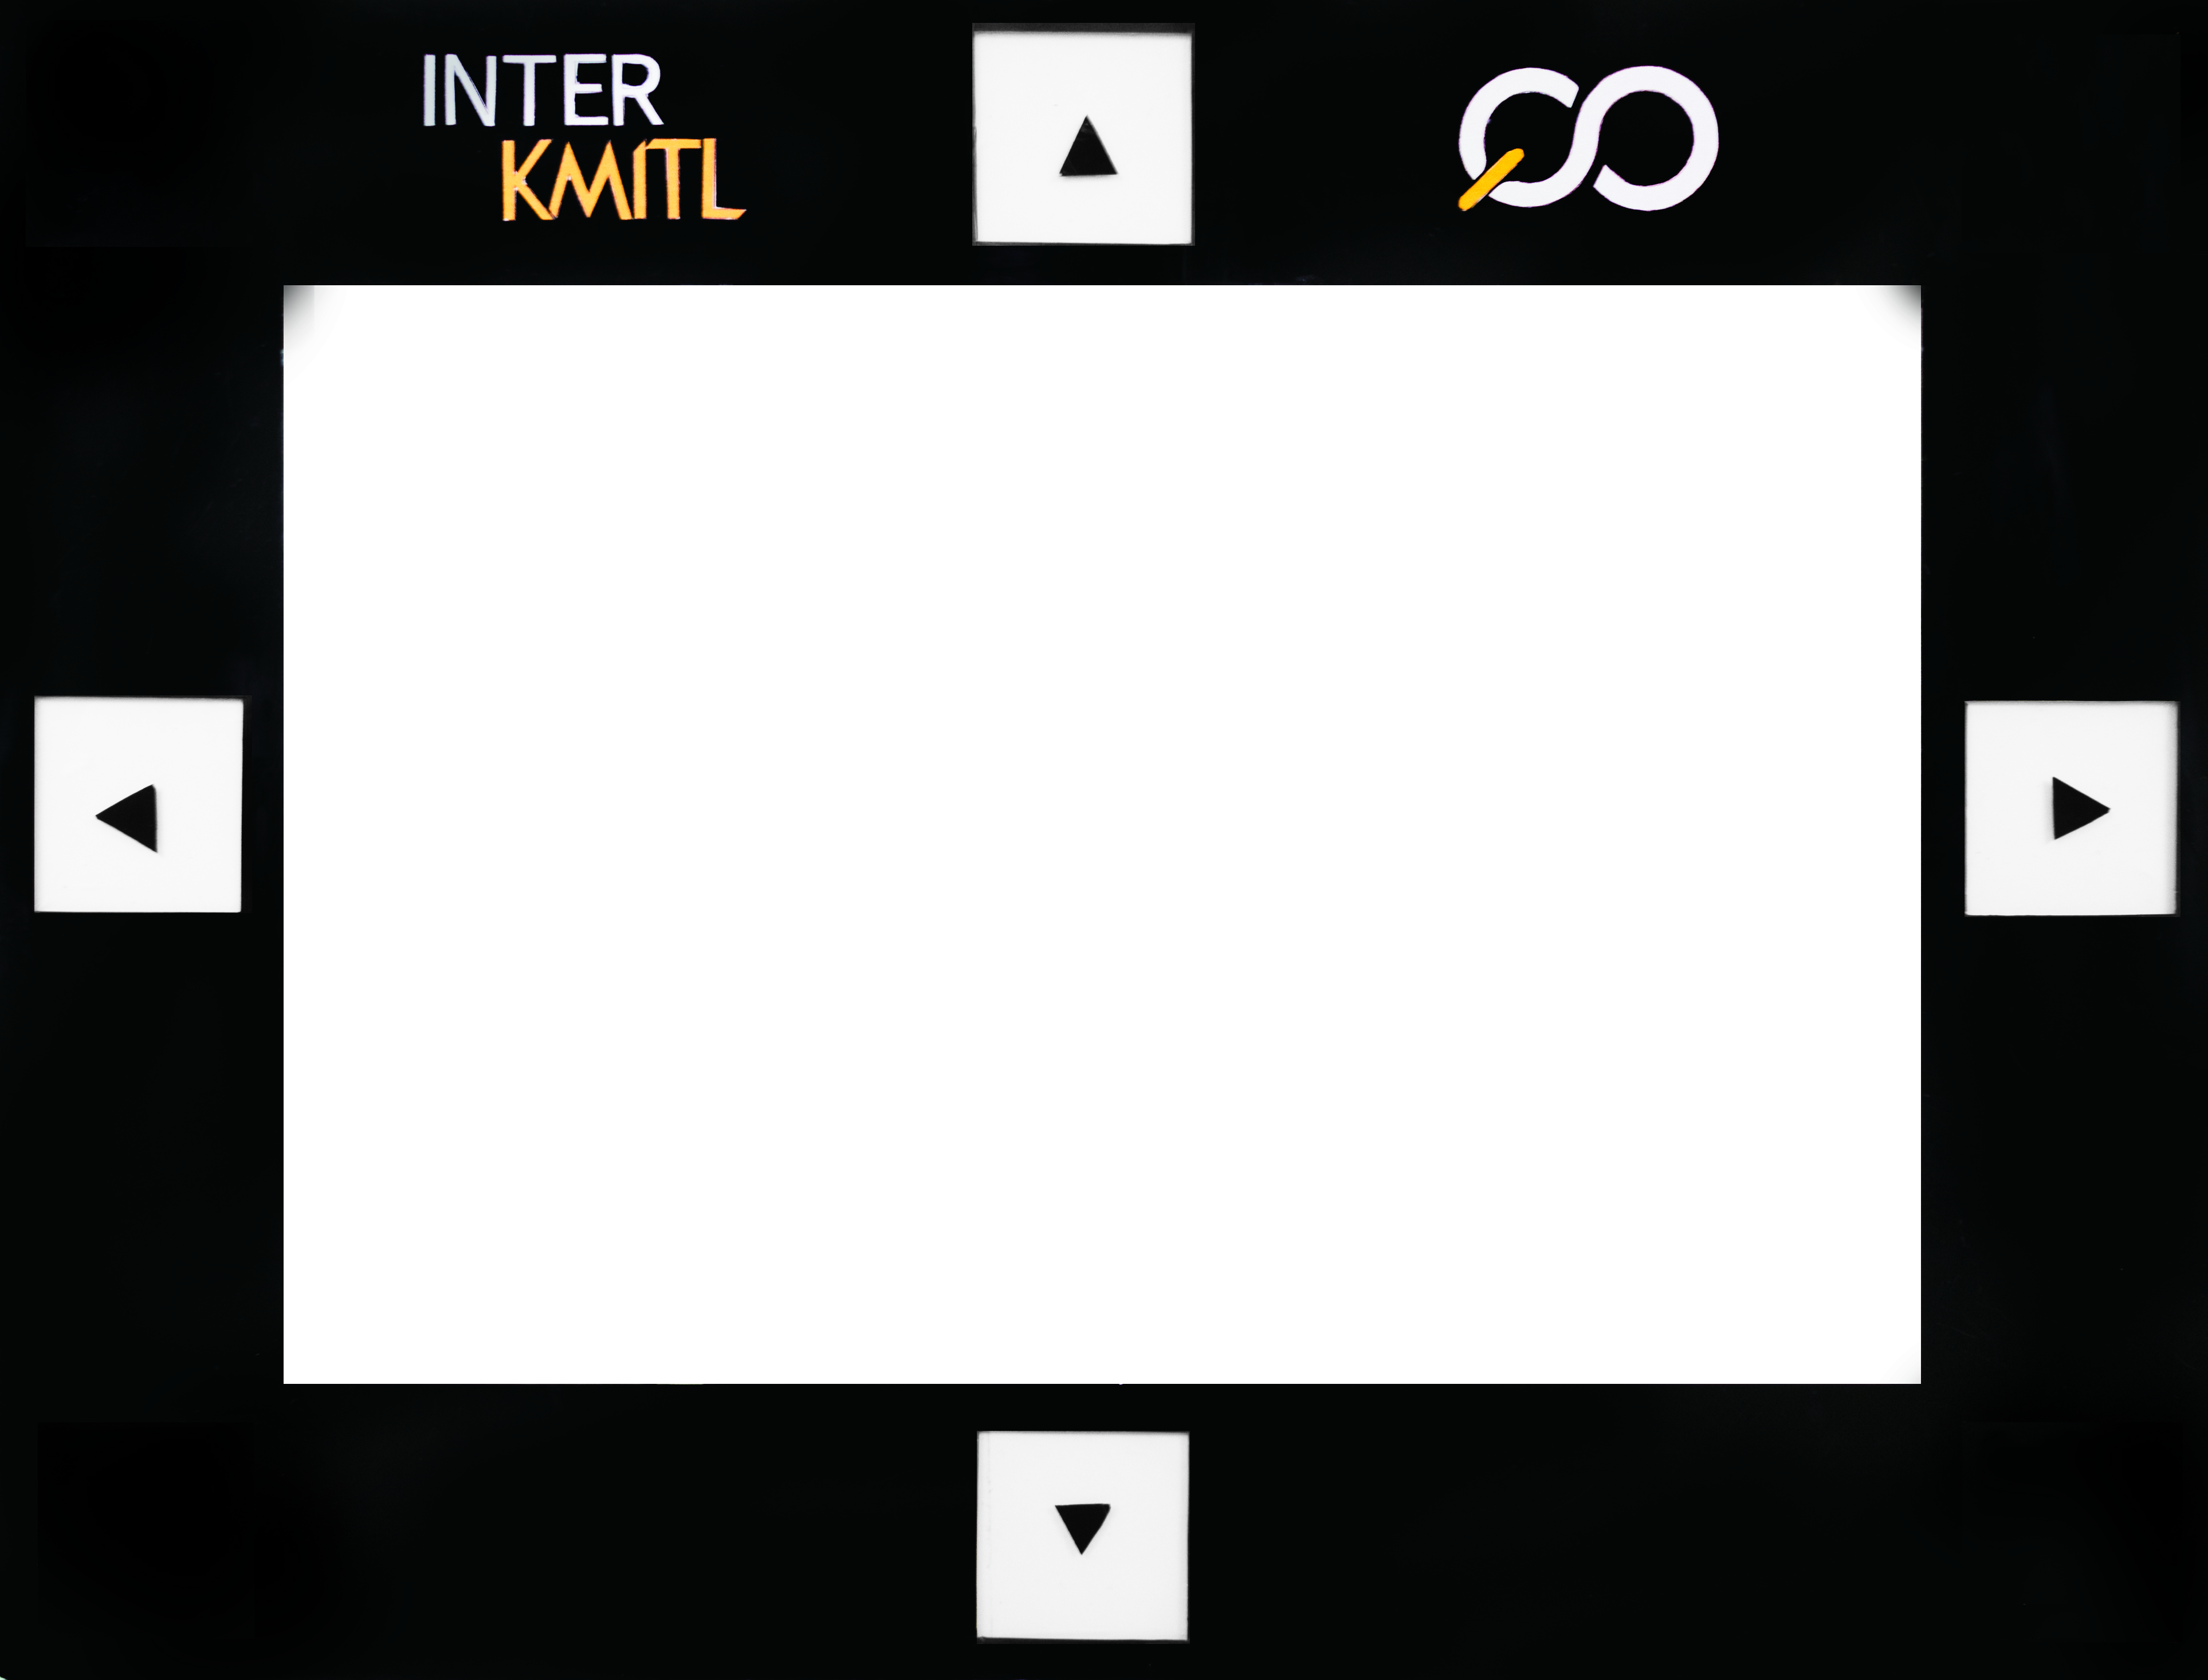
\includegraphics[scale=0.25]{chapter7/frame_4.jpg}
	\caption{Visual Stimulator with four targets used for ERPs}
\end{figure}

\newpage
\subsection{Visual stimulus (SSVEP)}
\hspace{1.5cm} This visual stimulator was developed based on the previous visual stimulus(ERP). The difference between this stimulator and previous stimulator is that, this stimulator has 8 flickers and each flicker has different frequencies, which was used in Experiment II and III.

\begin{figure}[ht]
	\centering
	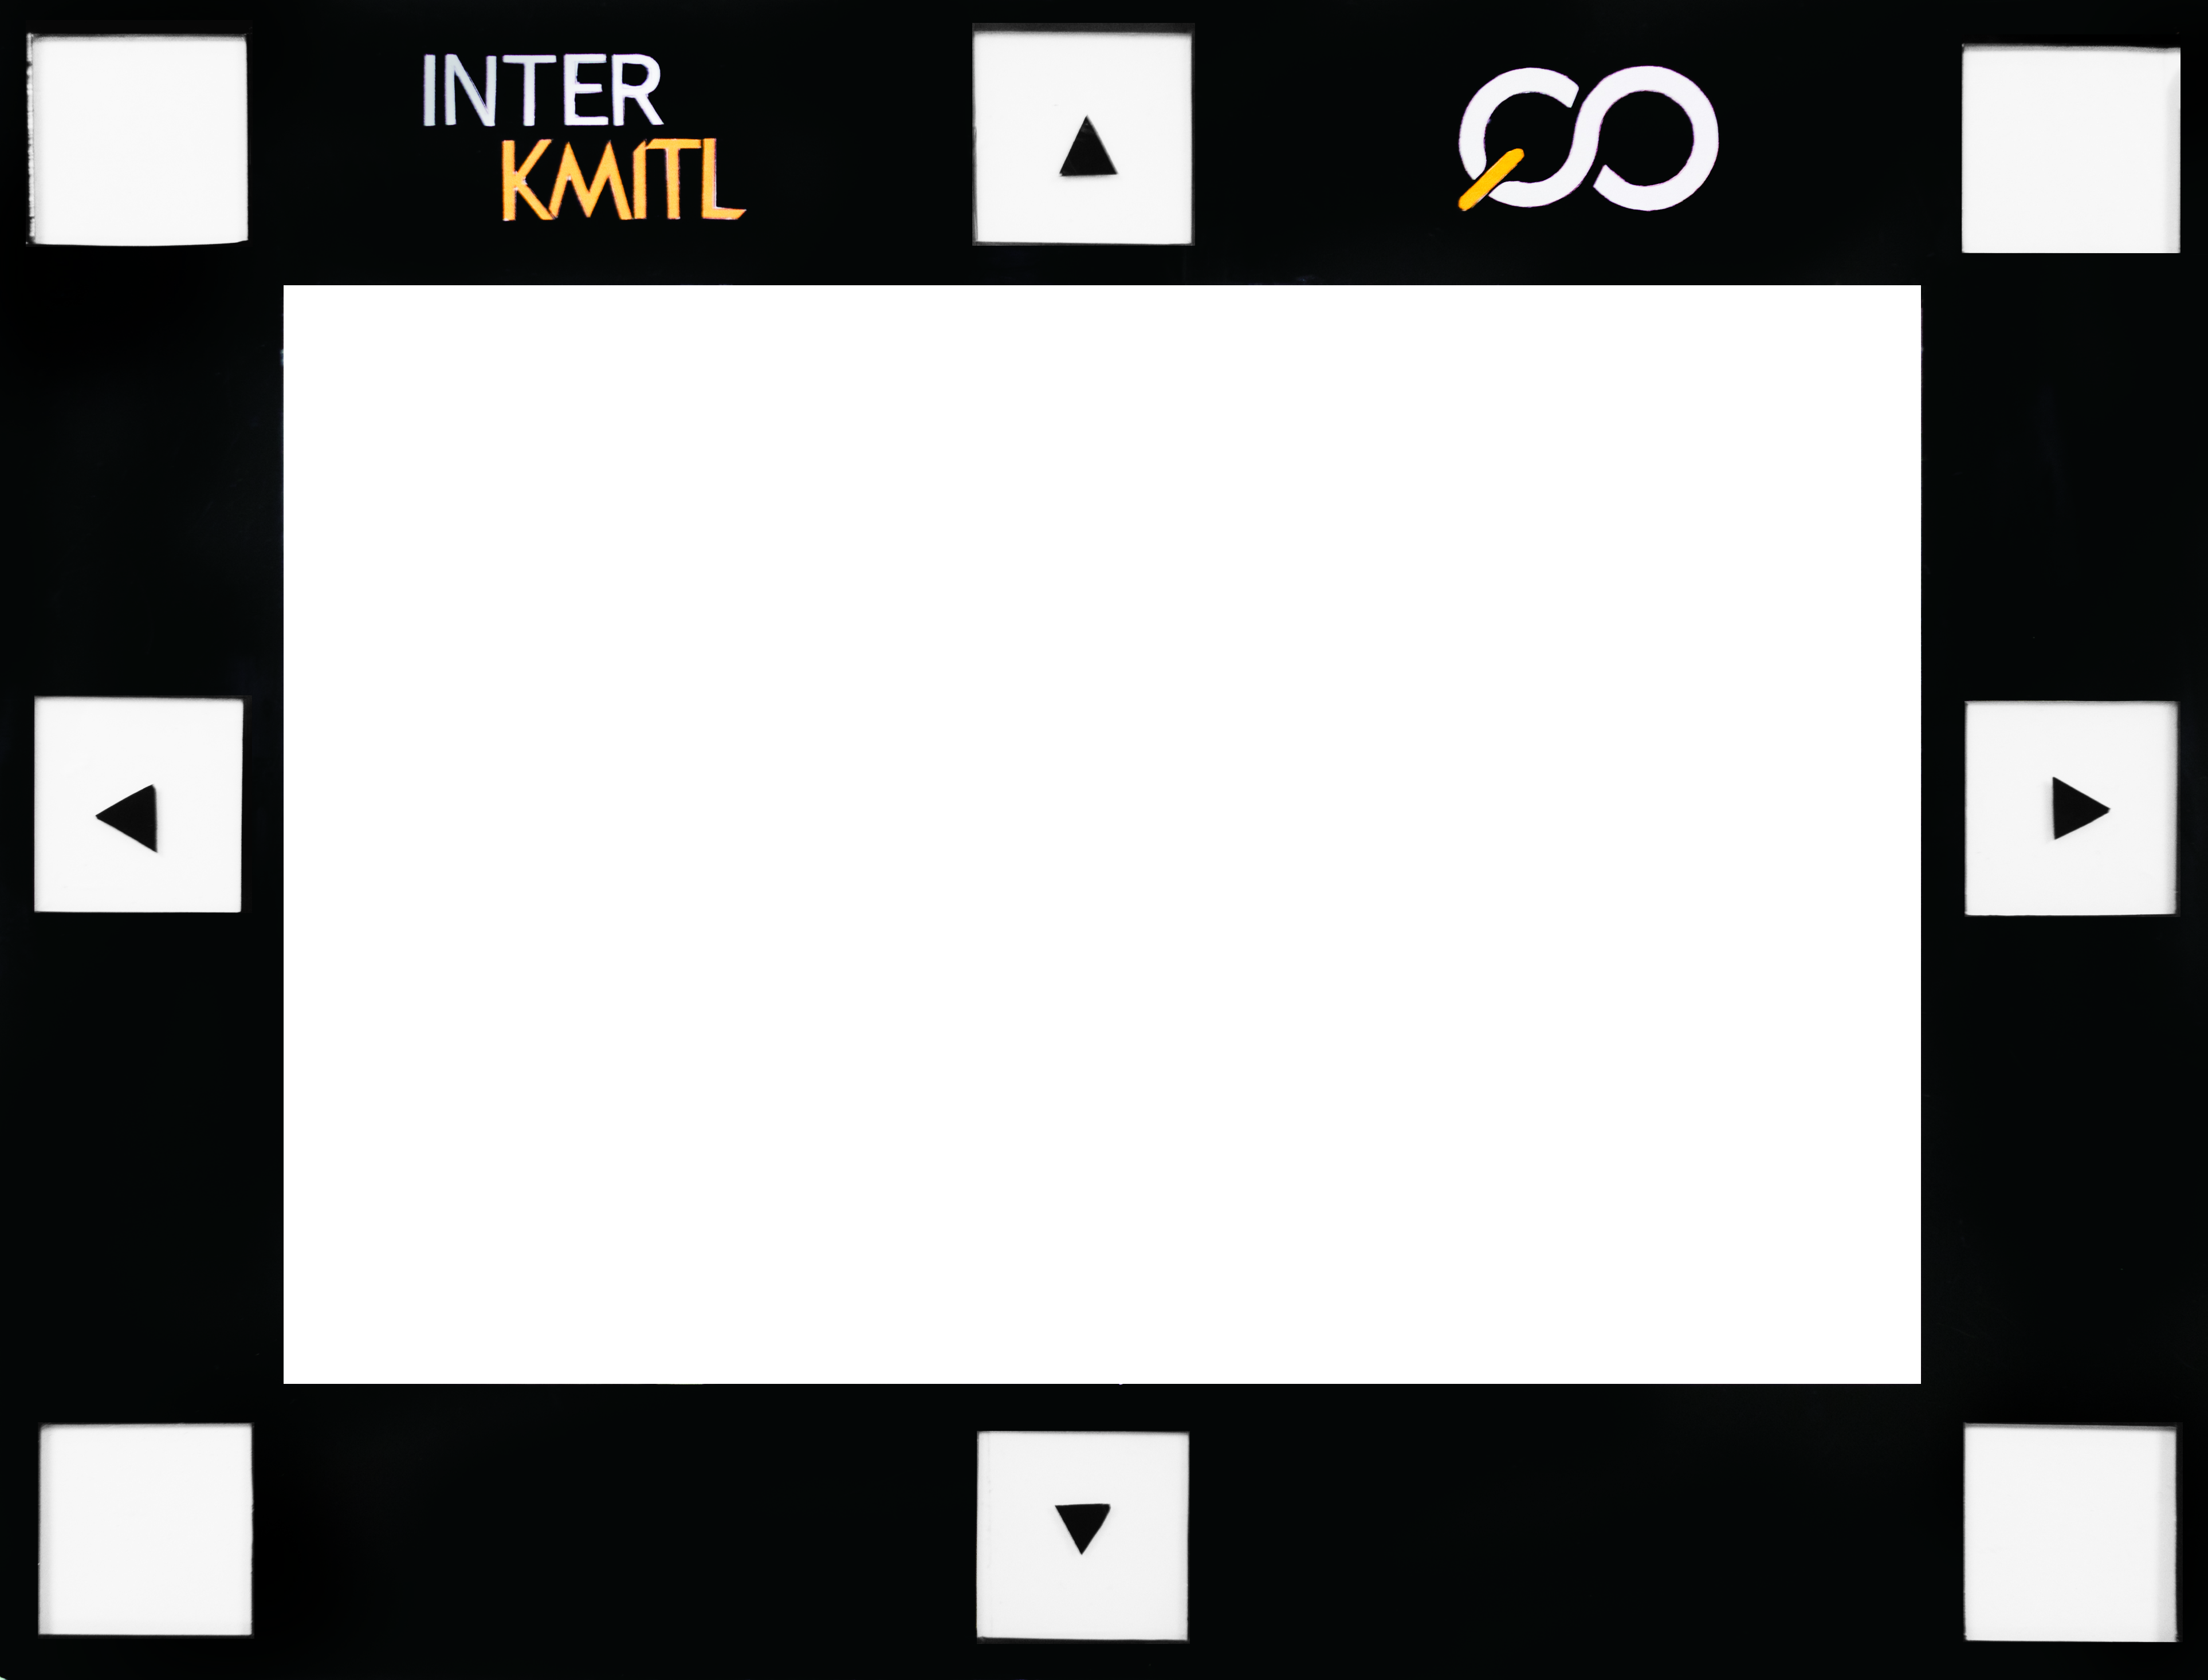
\includegraphics[scale=0.25]{chapter7/frame_8.jpg}
	\caption{Visual Stimulator with eight targets used for SSVEP}
\end{figure}

\newpage
\section{Experiment I}
\subsection{Experimental Paradigm I}
\begin{itemize}
\item{\textbf{Subjects}}\newline
In this experiment, we use 4 subjects. There are SS,OK,WP and NT that is the nickname and firstname of subjects.

\newcolumntype{P}[1]{>{\centering\arraybackslash}p{#1}}
\begin{table}[ht]
\centering
\begin{tabular}{| P{.2\linewidth} | P{.2\linewidth} | P{.2\linewidth} |}
			\hline 
			\textbf{Subjects} & \textbf{Age}  & \textbf{Sex}\\
			\hline 
			SS & 22 & Male\\
			\hline 
			OK & 22 & Male\\
			\hline 
			WP & 21 & Male\\
			\hline 
			NT & 21 & Male\\
			\hline
		\end{tabular}       
\caption{Experimental paradigm}
\label{table:2}
\end{table}

\item{\textbf{Stimulus}}
For one trial, we use 11, 15, 19, 23 seconds respectively.
\item{\textbf{Trials}}
We recorded 3, 5, 7, 9 times for each set of parameter.
\item{\textbf{Environment}}
In this experiment, we control the light illuminate value at 37 Lux.
	\item{\textbf{Parameters}}\\
There are 4 parameters. First is flickering type, stimulus, sample length and epoch time.
\end{itemize}

\newcolumntype{P}[1]{>{\centering\arraybackslash}p{#1}}
\begin{table}[ht]
\centering
\begin{tabular}{| P{.3\linewidth} | P{.3\linewidth} | P{.3\linewidth} |}
			
			\hline 
			\textbf{Parameter} & \textbf{Experiment1}  & \textbf{Experiment2}\\
			\hline 
            Stimulus & \multicolumn{2}{c}{Regualr} \vline\\
			\hline 
			Flickering type & Regular & Modulus   \\
			\hline 
			Sample Length & \multicolumn{2}{c}{64samples/epoch} \vline\\
			\hline 
			Epoch time & \multicolumn{2}{c}{500 ms} \vline\\
			\hline
		\end{tabular}       
\caption{Experimental paradigm}
\label{table:2}
\end{table}

In this experiment, we set duty-cycle be 0.7 and intensity to be 50\%. Experimental paradigm is shown in Table 7.1. We set the type of stimulus, sample length, epoch time, duty cycle, intensity and frequency to be the same. There are difference in flickering types. For first experiment, we blink regular flickers consecutively from LED1 to LED4, and the second experiment, uniform random is used to random the flickers. We have 3, 5, 7, and 9 trails for each subject to obtain the EEG. When we get the EEG, we take it to find average and accuracy of this experiment.

\newpage
\subsection{Experiment result I}

\hspace{1.5cm} From the figure 7.6, we obtain the EEG data of flickers line Y1,Y3,Y5 and Y7 for experiment I from trial= 3, subject = "OK". When we receive the EEG data of each flicker (Figure 7.6), we use range of 290-350 millisecond to classify which flicker that the subject fixate. From figure 7.6, we will see the 4 lines of graph. Y1 the EEG data from flicker 1, Y3 is from flicker 2, Y5 is from flicker3, and Y7 is from flicker 4. Each line means that we collect the data of the subject for 3 trials and compute the average of the EEG data that we got in each line. When we have already computed the average, we apply the normalization to all of the data which are averages to compare with each other. In this figure, the flicker that the subject fixate is Y5 or flicker 3.

\begin{figure}[ht]
	\centering
	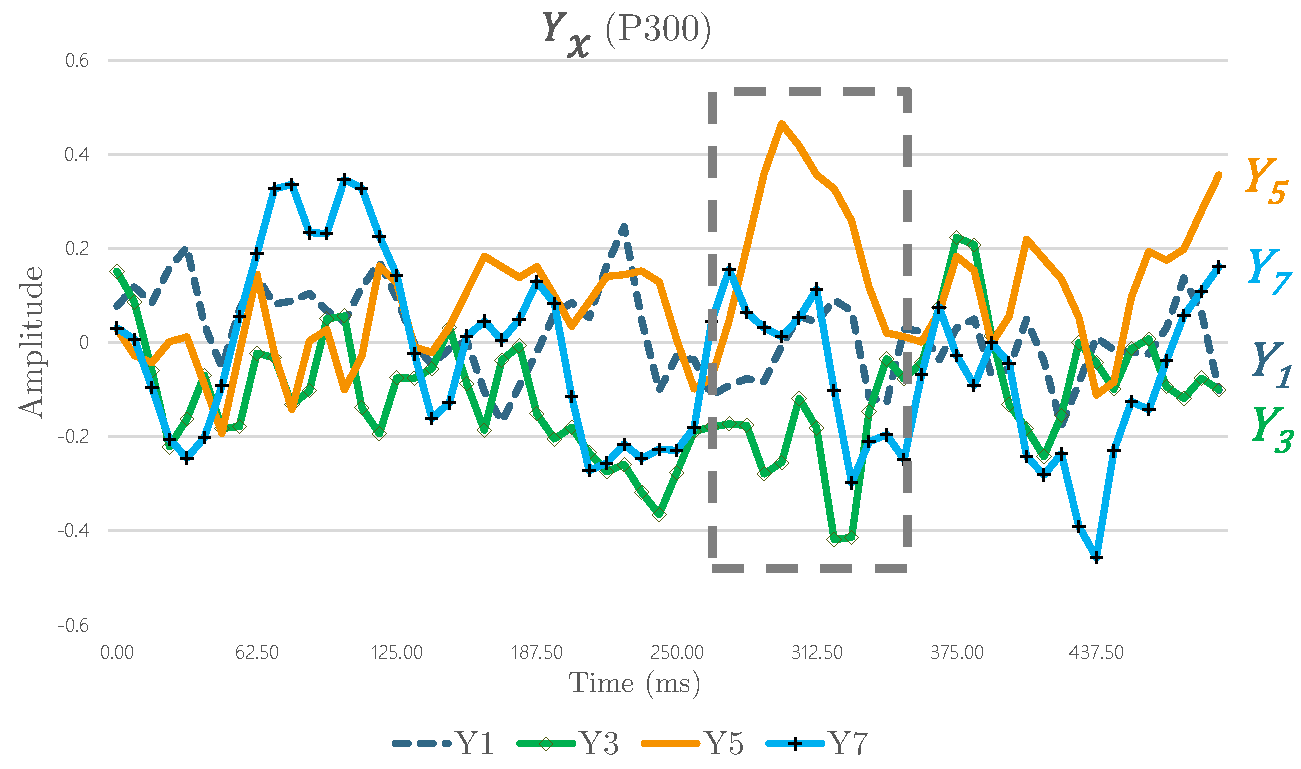
\includegraphics[width=\textwidth]{chapter7/erp_result.pdf}
	\caption{EEG data of subject "OK" ,trial = 3 from flickers Y1,Y3,Y5 and Y7}
\end{figure}

From the figure 7.7, we have a comparison graph of the first experiment EXP1 and the second experiment EXP2. Both are different in flickering types. EXP1's flickering type is regular, whereas EXP2 has a uniform random type. This graph display the accuracy of EXP1 and EXP2, where the trial = 7. The accuracy of EXP1 is equal to 70\% and EXP2 is equal to 80\%. We can see that EXP2 is more accurate than EXP1 in any trails that we use.

\begin{figure}[ht]
	\centering
	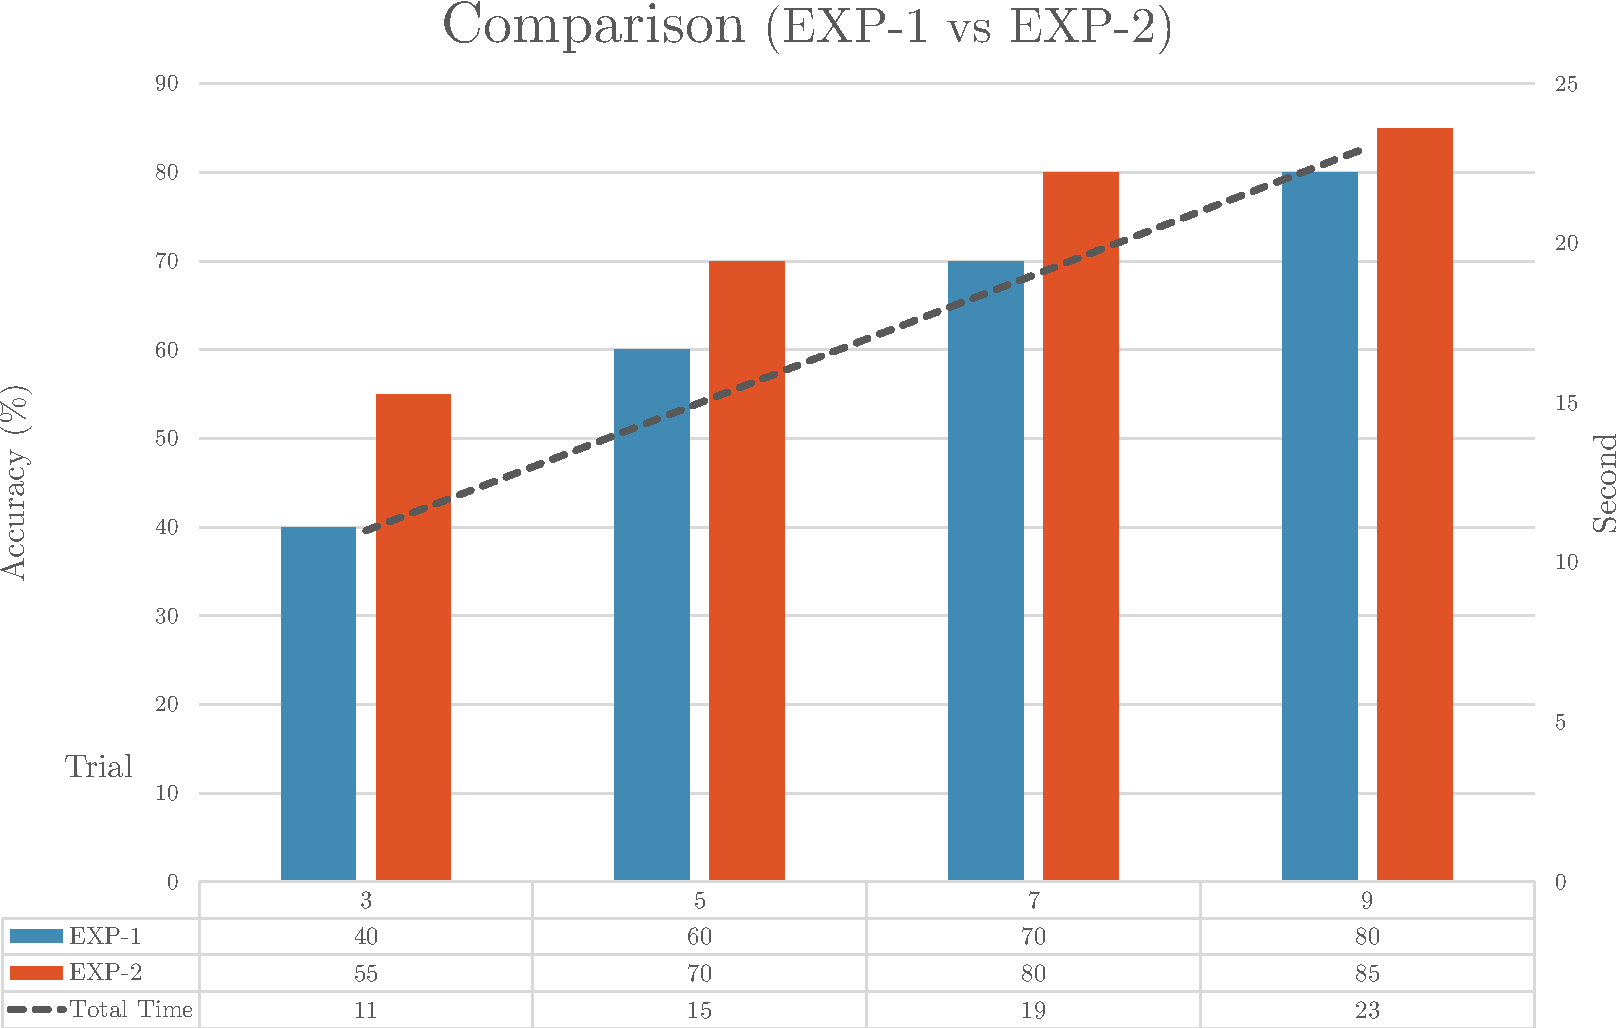
\includegraphics[width=\textwidth]{chapter7/result_12.pdf}
	\caption{Comparison between the result of experiment1 and 2}
\end{figure}

\begin{table}[ht]
\centering
\resizebox{\textwidth}{!}{
\begin{tabular}{| c | c | c | c | c |}

			\hline 
			\multirow{2}{*}{\textbf{Trial}} & 
  			\multirow{2}{*}{\textbf{Total time [s]}}  & 
            \multirow{2}{*}{\textbf{Subject}} &
            \multicolumn{2}{c|}{\textbf{Accuracy of flickering type}} \\
            \cline{4-5}
            &&&\multicolumn{1}{c|}{\textbf{Regular}} &\multicolumn{1}{c|}{\textbf{Uniform}}  \\
			\hline 
			\multirow{4}{*}{3}&\multirow{4}{*}{11}&OK&30&60 \\
			\cline{3-5}
			&&WP&50&65 \\ \cline{3-5}
			&&SS&45&50 \\ \cline{3-5}
			&&NT&35&45 \\
            \hline
			\multirow{4}{*}{5}&\multirow{4}{*}{15}&OK&55&75 \\
			\cline{3-5}
			&&WP&60&70 \\ \cline{3-5}
			&&SS&65&70 \\ \cline{3-5}
			&&NT&60&65 \\
            \hline
            \multirow{4}{*}{7}&\multirow{4}{*}{19}&OK&70&75 \\
			\cline{3-5}
			&&WP&80&80 \\ \cline{3-5}
			&&SS&65&85 \\ \cline{3-5}
			&&NT&65&80 \\
            \hline 
            \multirow{4}{*}{9}&\multirow{4}{*}{23}&OK&85&85 \\
			\cline{3-5}
			&&WP&80&90 \\ \cline{3-5}
			&&SS&75&80 \\ \cline{3-5}
			&&NT&80&85 \\
            \hline 
		\end{tabular}       
        }
\caption{Experiment result}
\label{table:3}
\end{table}

The result of this experiment is shown in Table 7.2 with same set of parameter for each stimulus, sample length, epoch time, duty cycle, intensity and frequency. First from the Table 7.2, we compare between regular and uniform random.In the first row we can see the accuracy of "OK" in uniform random is better than regular and "NT" in the last row we can see the accuracy of uniform random is better than regular too. We found each subject have better accuracy in uniform random than regular of flickering type.We found the other thing that is the trial of the experiment. We will compare between "WP" in second row and "WP" in tenth row.The accuracy of "WP" in tenth row is better than "WP" in second row. The main factor is trial that we use in each experiment. We found that when we use more trials, the accuracy is increased too.

\newpage
\section{Experiment II}
\subsection{Experimental Paradigm I}
\begin{itemize}
\item{\textbf{Subjects}}\newline
In this experiment, we use 4 subjects. There are SS,OK,WP and NT that is the nickname and firstname of subjects.

\newcolumntype{P}[1]{>{\centering\arraybackslash}p{#1}}
\begin{table}[ht]
\centering
\begin{tabular}{| P{.2\linewidth} | P{.2\linewidth} | P{.2\linewidth} |}
			\hline 
			\textbf{Subjects} & \textbf{Age}  & \textbf{Sex}\\
			\hline 
			SS & 22 & Male\\
			\hline 
			OK & 22 & Male\\
			\hline 
			WP & 21 & Male\\
			\hline 
			NT & 21 & Male\\
			\hline
		\end{tabular}       
\caption{Experimental paradigm}
\label{table:2}
\end{table}

\item{\textbf{Stimulus}}
For one trial, we use 11, 15, 19, 23 seconds respectively.
\item{\textbf{Trials}}
We recorded 3, 5, 7, 9 times for each set of parameter.
\item{\textbf{Environment}}
In this experiment, we control the light illuminate value at 37 Lux.
	\item{\textbf{Parameters}}\\
There are 4 parameters. First is flickering type, stimulus, sample length and epoch time.
\end{itemize}

\newcolumntype{P}[1]{>{\centering\arraybackslash}p{#1}}
\begin{table}[ht]
\centering
\begin{tabular}{| P{.3\linewidth} | P{.3\linewidth} | P{.3\linewidth} |}
			
			\hline 
			\textbf{Parameter} & \textbf{Experiment1}  & \textbf{Experiment2}\\
			\hline 
			Flickering type & Regular & Uniform random   \\
			\hline 
			Stimulus & \multicolumn{2}{c}{Modular} \vline\\
			\hline 
			Sample Length & \multicolumn{2}{c}{64samples/epoch} \vline\\
			\hline 
			Epoch time & \multicolumn{2}{c}{500 ms} \vline\\
			\hline
		\end{tabular}       
\caption{Experimental paradigm}
\label{table:2}
\end{table}

In this experiment, we set duty-cycle be 0.7 and intensity to be 50\%. Experimental paradigm is shown in Table 7.1. We set the type of stimulus, sample length, epoch time, duty cycle, intensity and frequency to be the same. There are difference in flickering types. For first experiment, we blink regular flickers consecutively from LED1 to LED4, and the second experiment, uniform random is used to random the flickers. We have 3, 5, 7, and 9 trails for each subject to obtain the EEG. When we get the EEG, we take it to find average and accuracy of this experiment.

\newpage
\subsection{Experiment result I}

\hspace{1.5cm} From the figure 7.6, we obtain the EEG data of flickers line Y1,Y3,Y5 and Y7 for experiment I from trial= 3, subject = "OK". When we receive the EEG data of each flicker (Figure 7.6), we use range of 290-350 millisecond to classify which flicker that the subject fixate. From figure 7.6, we will see the 4 lines of graph. Y1 the EEG data from flicker 1, Y3 is from flicker 2, Y5 is from flicker3, and Y7 is from flicker 4. Each line means that we collect the data of the subject for 3 trials and compute the average of the EEG data that we got in each line. When we have already computed the average, we apply the normalization to all of the data which are averages to compare with each other. In this figure, the flicker that the subject fixate is Y5 or flicker 3.

\begin{figure}[ht]
	\centering
	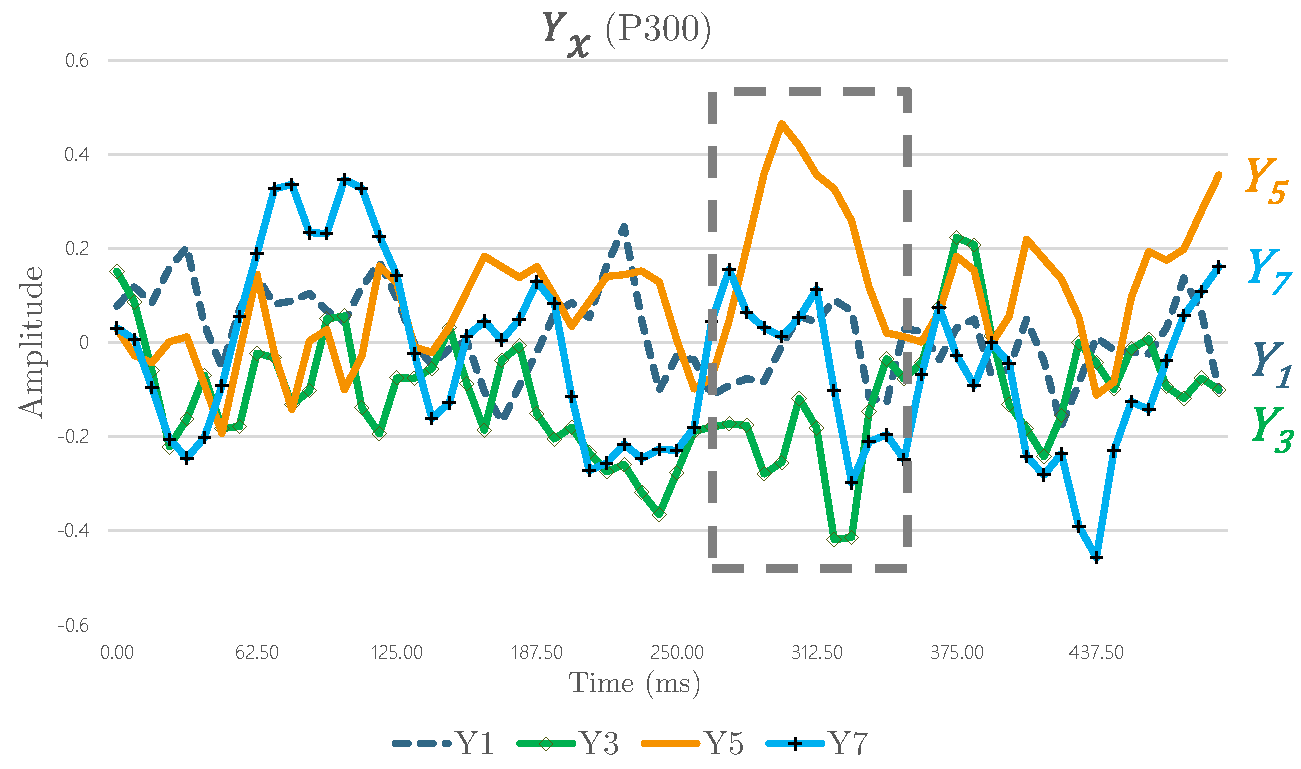
\includegraphics[width=\textwidth]{chapter7/erp_result.pdf}
	\caption{EEG data of subject "OK" ,trial = 3 from flickers Y1,Y3,Y5 and Y7}
\end{figure}

From the figure 7.7, we have a comparison graph of the first experiment EXP1 and the second experiment EXP2. Both are different in flickering types. EXP1's flickering type is regular, whereas EXP2 has a uniform random type. This graph display the accuracy of EXP1 and EXP2, where the trial = 7. The accuracy of EXP1 is equal to 70\% and EXP2 is equal to 80\%. We can see that EXP2 is more accurate than EXP1 in any trails that we use.

\begin{figure}[ht]
	\centering
	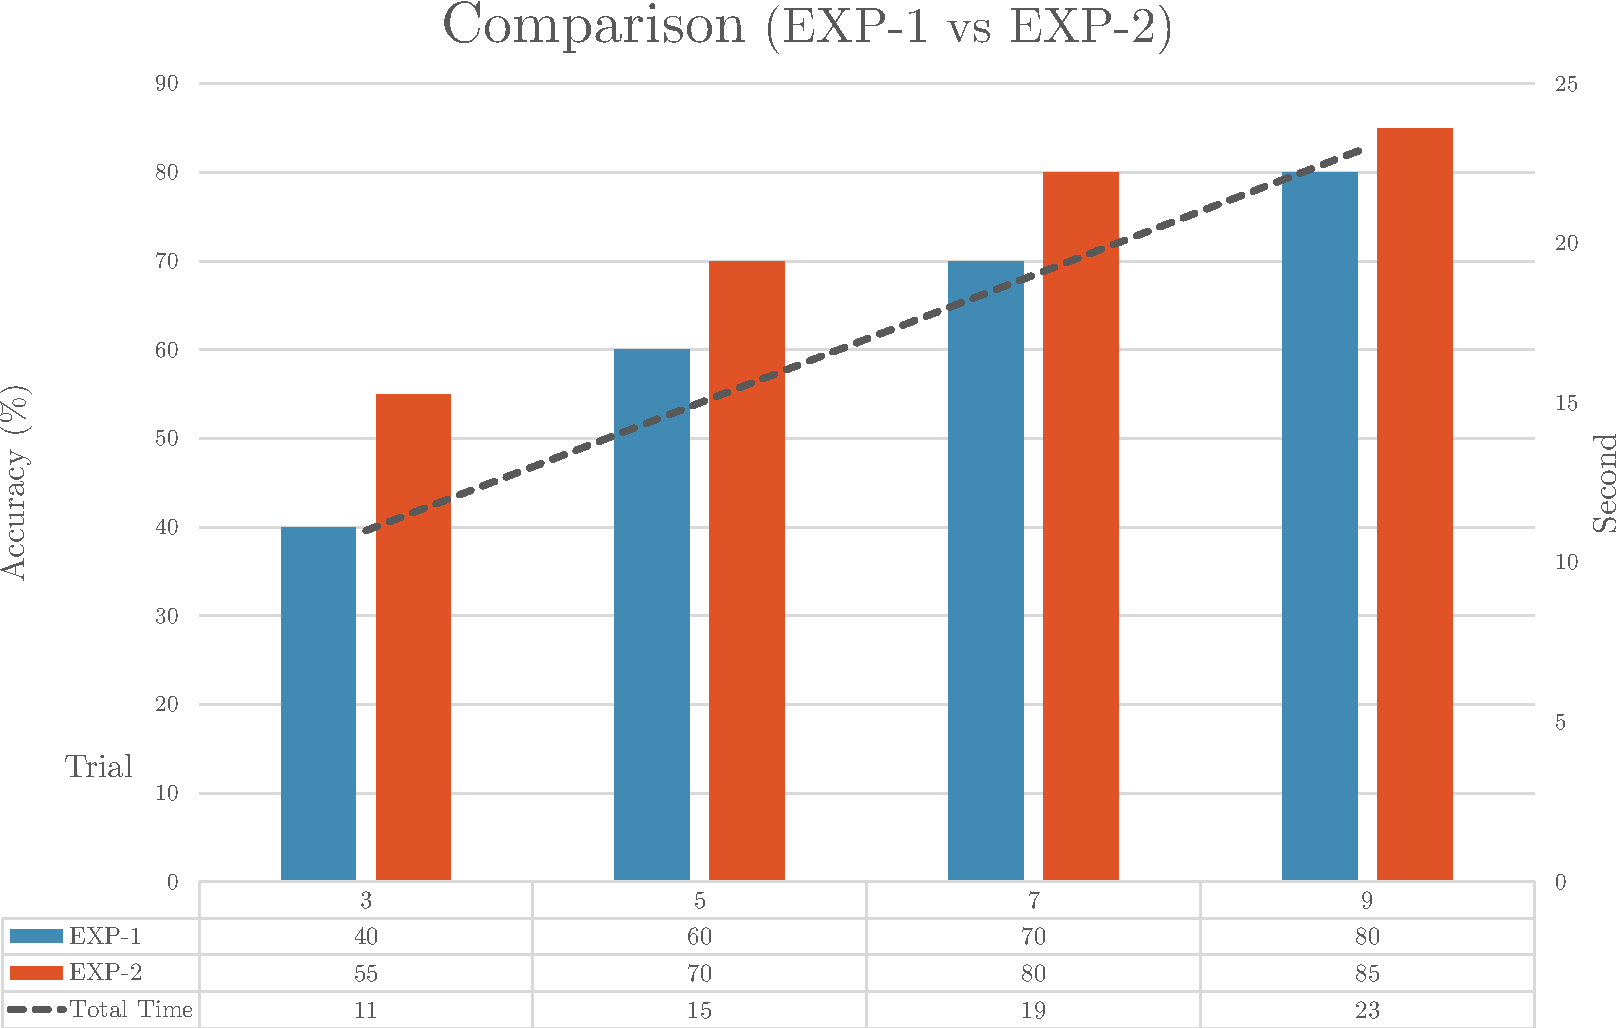
\includegraphics[width=\textwidth]{chapter7/result_12.pdf}
	\caption{Comparison between the result of experiment1 and 2}
\end{figure}

\begin{table}[ht]
\centering
\resizebox{\textwidth}{!}{
\begin{tabular}{| c | c | c | c | c |}

			\hline 
			\multirow{2}{*}{\textbf{Trial}} & 
  			\multirow{2}{*}{\textbf{Total time [s]}}  & 
            \multirow{2}{*}{\textbf{Subject}} &
            \multicolumn{2}{c|}{\textbf{Accuracy of flickering type}} \\
            \cline{4-5}
            &&&\multicolumn{1}{c|}{\textbf{Regular}} &\multicolumn{1}{c|}{\textbf{Uniform}}  \\
			\hline 
			\multirow{4}{*}{3}&\multirow{4}{*}{11}&OK&30&60 \\
			\cline{3-5}
			&&WP&50&65 \\ \cline{3-5}
			&&SS&45&50 \\ \cline{3-5}
			&&NT&35&45 \\
            \hline
			\multirow{4}{*}{5}&\multirow{4}{*}{15}&OK&55&75 \\
			\cline{3-5}
			&&WP&60&70 \\ \cline{3-5}
			&&SS&65&70 \\ \cline{3-5}
			&&NT&60&65 \\
            \hline
            \multirow{4}{*}{7}&\multirow{4}{*}{19}&OK&70&75 \\
			\cline{3-5}
			&&WP&80&80 \\ \cline{3-5}
			&&SS&65&85 \\ \cline{3-5}
			&&NT&65&80 \\
            \hline 
            \multirow{4}{*}{9}&\multirow{4}{*}{23}&OK&85&85 \\
			\cline{3-5}
			&&WP&80&90 \\ \cline{3-5}
			&&SS&75&80 \\ \cline{3-5}
			&&NT&80&85 \\
            \hline 
		\end{tabular}       
        }
\caption{Experiment result}
\label{table:3}
\end{table}

The result of this experiment is shown in Table 7.2 with same set of parameter for each stimulus, sample length, epoch time, duty cycle, intensity and frequency. First from the Table 7.2, we compare between regular and uniform random.In the first row we can see the accuracy of "OK" in uniform random is better than regular and "NT" in the last row we can see the accuracy of uniform random is better than regular too. We found each subject have better accuracy in uniform random than regular of flickering type.We found the other thing that is the trial of the experiment. We will compare between "WP" in second row and "WP" in tenth row.The accuracy of "WP" in tenth row is better than "WP" in second row. The main factor is trial that we use in each experiment. We found that when we use more trials, the accuracy is increased too.


























